\documentclass[man,floatsintext]{apa6}
\usepackage{lmodern}
\usepackage{amssymb,amsmath}
\usepackage{ifxetex,ifluatex}
\usepackage{fixltx2e} % provides \textsubscript
\ifnum 0\ifxetex 1\fi\ifluatex 1\fi=0 % if pdftex
  \usepackage[T1]{fontenc}
  \usepackage[utf8]{inputenc}
\else % if luatex or xelatex
  \ifxetex
    \usepackage{mathspec}
  \else
    \usepackage{fontspec}
  \fi
  \defaultfontfeatures{Ligatures=TeX,Scale=MatchLowercase}
\fi
% use upquote if available, for straight quotes in verbatim environments
\IfFileExists{upquote.sty}{\usepackage{upquote}}{}
% use microtype if available
\IfFileExists{microtype.sty}{%
\usepackage{microtype}
\UseMicrotypeSet[protrusion]{basicmath} % disable protrusion for tt fonts
}{}
\usepackage{hyperref}
\hypersetup{unicode=true,
            pdftitle={What explains happiness? The relationships between happiness and marrige, religion health, trust, and saving},
            pdfauthor={Asha, Joanna, \& Thuy},
            pdfkeywords={happiness},
            pdfborder={0 0 0},
            breaklinks=true}
\urlstyle{same}  % don't use monospace font for urls
\usepackage{graphicx,grffile}
\makeatletter
\def\maxwidth{\ifdim\Gin@nat@width>\linewidth\linewidth\else\Gin@nat@width\fi}
\def\maxheight{\ifdim\Gin@nat@height>\textheight\textheight\else\Gin@nat@height\fi}
\makeatother
% Scale images if necessary, so that they will not overflow the page
% margins by default, and it is still possible to overwrite the defaults
% using explicit options in \includegraphics[width, height, ...]{}
\setkeys{Gin}{width=\maxwidth,height=\maxheight,keepaspectratio}
\IfFileExists{parskip.sty}{%
\usepackage{parskip}
}{% else
\setlength{\parindent}{0pt}
\setlength{\parskip}{6pt plus 2pt minus 1pt}
}
\setlength{\emergencystretch}{3em}  % prevent overfull lines
\providecommand{\tightlist}{%
  \setlength{\itemsep}{0pt}\setlength{\parskip}{0pt}}
\setcounter{secnumdepth}{0}
% Redefines (sub)paragraphs to behave more like sections
\ifx\paragraph\undefined\else
\let\oldparagraph\paragraph
\renewcommand{\paragraph}[1]{\oldparagraph{#1}\mbox{}}
\fi
\ifx\subparagraph\undefined\else
\let\oldsubparagraph\subparagraph
\renewcommand{\subparagraph}[1]{\oldsubparagraph{#1}\mbox{}}
\fi

%%% Use protect on footnotes to avoid problems with footnotes in titles
\let\rmarkdownfootnote\footnote%
\def\footnote{\protect\rmarkdownfootnote}


  \title{What explains happiness? The relationships between happiness and
marrige, religion health, trust, and saving}
    \author{Asha\textsuperscript{1}, Joanna\textsuperscript{1}, \&
Thuy\textsuperscript{1}}
    \date{}
  
\shorttitle{What explains happiness?}
\affiliation{
\vspace{0.5cm}
\textsuperscript{1} University of Oregon}
\keywords{happiness\newline\indent Word count: X}
\usepackage{csquotes}
\usepackage{upgreek}
\captionsetup{font=singlespacing,justification=justified}

\usepackage{longtable}
\usepackage{lscape}
\usepackage{multirow}
\usepackage{tabularx}
\usepackage[flushleft]{threeparttable}
\usepackage{threeparttablex}

\newenvironment{lltable}{\begin{landscape}\begin{center}\begin{ThreePartTable}}{\end{ThreePartTable}\end{center}\end{landscape}}

\makeatletter
\newcommand\LastLTentrywidth{1em}
\newlength\longtablewidth
\setlength{\longtablewidth}{1in}
\newcommand{\getlongtablewidth}{\begingroup \ifcsname LT@\roman{LT@tables}\endcsname \global\longtablewidth=0pt \renewcommand{\LT@entry}[2]{\global\advance\longtablewidth by ##2\relax\gdef\LastLTentrywidth{##2}}\@nameuse{LT@\roman{LT@tables}} \fi \endgroup}


\usepackage{lineno}

\linenumbers

\authornote{We thank Dr.~Nese for his guidance in this
project. All mistakes remain ours.

Correspondence concerning this article should be addressed to Asha,
Postal address. E-mail:
\href{mailto:my@email.com}{\nolinkurl{my@email.com}}}

\abstract{
abstract goes here


}

\begin{document}
\maketitle

\begin{verbatim}
## [1] "Rather happy"                                                             
## [2] "Very happy"                                                               
## [3] "Not very happy"                                                           
## [4] "Not at all happy"                                                         
## [5] "No answer"                                                                
## [6] "Dont know"                                                                
## [7] "HT: Missing-Dropped out survey; RU: Inappropriate response{Inappropriate}"
\end{verbatim}

\begin{tabular}{l|l|r}
\hline
family\_savings & feeling\_of\_happiness & n\\
\hline
Just get by & Not at all happy & 813\\
\hline
Just get by & Not very happy & 4650\\
\hline
Just get by & Rather happy & 18661\\
\hline
Just get by & Very happy & 10545\\
\hline
Save money & Not at all happy & 203\\
\hline
Save money & Not very happy & 1449\\
\hline
Save money & Rather happy & 11060\\
\hline
Save money & Very happy & 9177\\
\hline
Spent savings and borrowed money & Not at all happy & 400\\
\hline
Spent savings and borrowed money & Not very happy & 1577\\
\hline
Spent savings and borrowed money & Rather happy & 3867\\
\hline
Spent savings and borrowed money & Very happy & 2489\\
\hline
Spent some savings and borrowed money & Not at all happy & 207\\
\hline
Spent some savings and borrowed money & Not very happy & 1471\\
\hline
Spent some savings and borrowed money & Rather happy & 5853\\
\hline
Spent some savings and borrowed money & Very happy & 3800\\
\hline
\end{tabular}

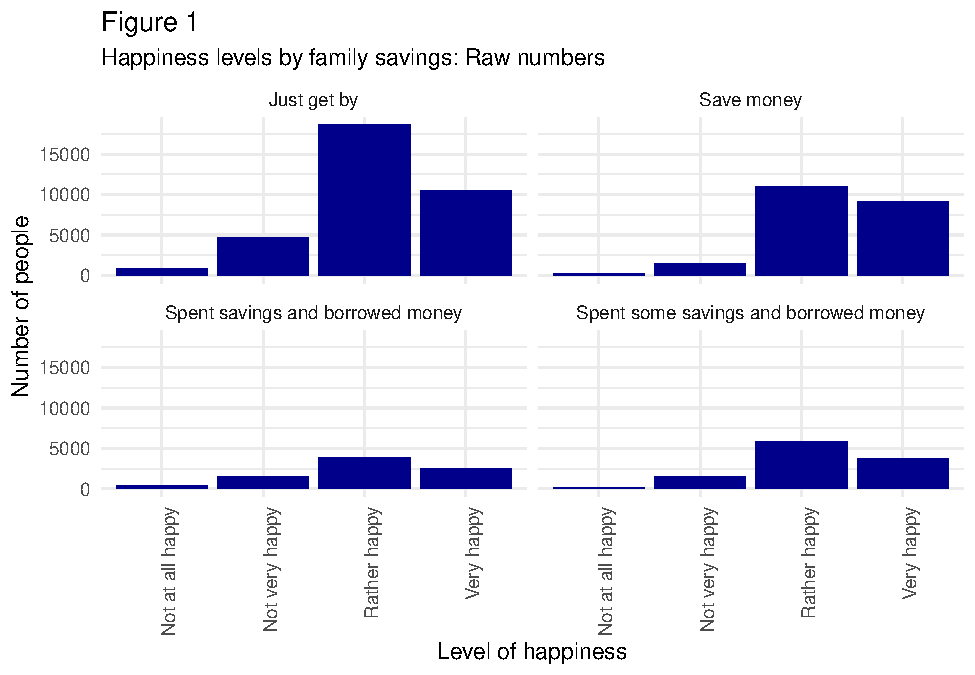
\includegraphics{610_final_files/figure-latex/happiness and family savings JW-1.pdf}
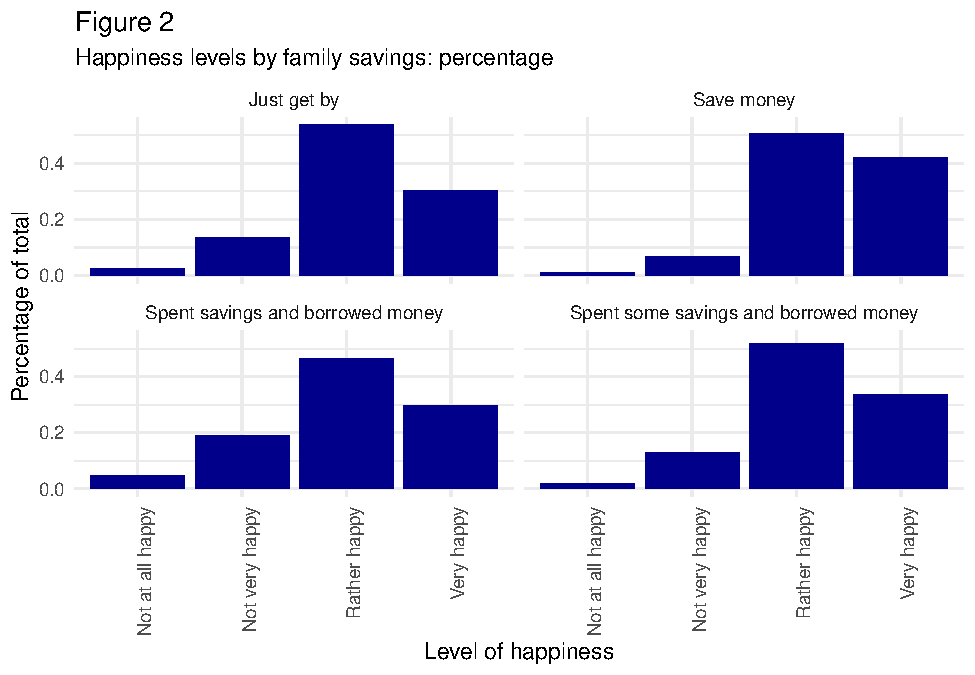
\includegraphics{610_final_files/figure-latex/happiness and family savings JW-2.pdf}

\begin{verbatim}
## # A tibble: 16 x 5
##    family_savings                   feeling_of_happine~     n total percent
##    <fct>                            <fct>               <int> <int>   <dbl>
##  1 Save money                       Not at all happy      203 21889 0.00927
##  2 Spent some savings and borrowed~ Not at all happy      207 11331 0.0183 
##  3 Just get by                      Not at all happy      813 34669 0.0235 
##  4 Spent savings and borrowed money Not at all happy      400  8333 0.0480 
##  5 Save money                       Not very happy       1449 21889 0.0662 
##  6 Spent some savings and borrowed~ Not very happy       1471 11331 0.130  
##  7 Just get by                      Not very happy       4650 34669 0.134  
##  8 Spent savings and borrowed money Not very happy       1577  8333 0.189  
##  9 Spent savings and borrowed money Very happy           2489  8333 0.299  
## 10 Just get by                      Very happy          10545 34669 0.304  
## 11 Spent some savings and borrowed~ Very happy           3800 11331 0.335  
## 12 Save money                       Very happy           9177 21889 0.419  
## 13 Spent savings and borrowed money Rather happy         3867  8333 0.464  
## 14 Save money                       Rather happy        11060 21889 0.505  
## 15 Spent some savings and borrowed~ Rather happy         5853 11331 0.517  
## 16 Just get by                      Rather happy        18661 34669 0.538
\end{verbatim}

\begin{figure}
\centering
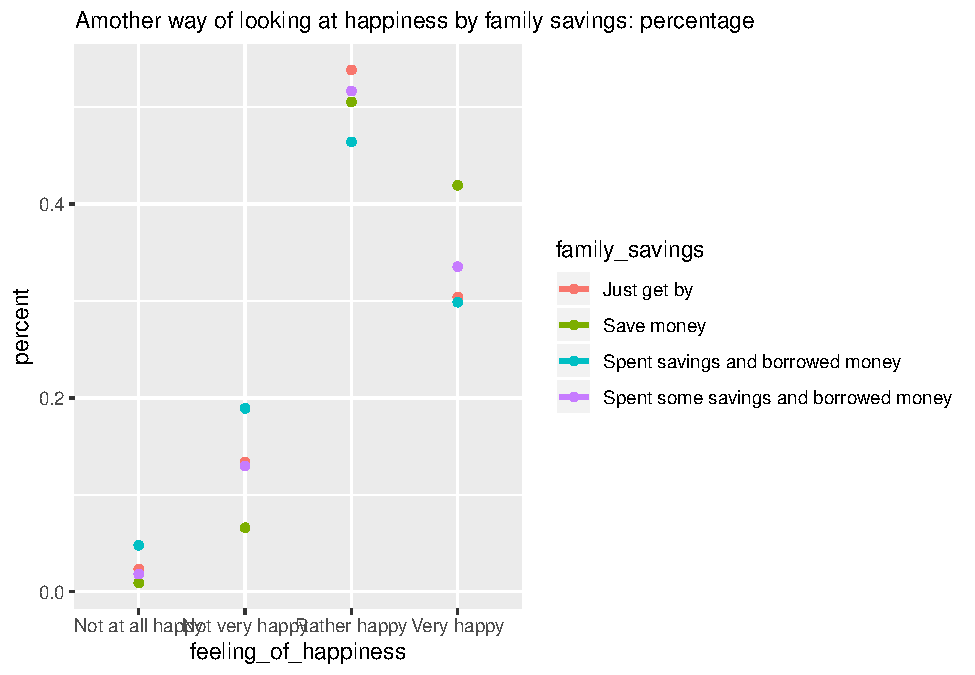
\includegraphics{610_final_files/figure-latex/happiness and family savings JW-3.pdf}
\caption{}
\end{figure}

\begin{verbatim}
## List of 65
##  $ line                      :List of 6
##   ..$ colour       : chr "black"
##   ..$ size         : num 0.5
##   ..$ linetype     : num 1
##   ..$ lineend      : chr "butt"
##   ..$ arrow        : logi FALSE
##   ..$ inherit.blank: logi TRUE
##   ..- attr(*, "class")= chr [1:2] "element_line" "element"
##  $ rect                      :List of 5
##   ..$ fill         : chr "white"
##   ..$ colour       : chr "black"
##   ..$ size         : num 0.5
##   ..$ linetype     : num 1
##   ..$ inherit.blank: logi TRUE
##   ..- attr(*, "class")= chr [1:2] "element_rect" "element"
##  $ text                      :List of 11
##   ..$ family       : chr ""
##   ..$ face         : chr "plain"
##   ..$ colour       : chr "black"
##   ..$ size         : num 11
##   ..$ hjust        : num 0.5
##   ..$ vjust        : num 0.5
##   ..$ angle        : num 0
##   ..$ lineheight   : num 0.9
##   ..$ margin       : 'margin' num [1:4] 0pt 0pt 0pt 0pt
##   .. ..- attr(*, "valid.unit")= int 8
##   .. ..- attr(*, "unit")= chr "pt"
##   ..$ debug        : logi FALSE
##   ..$ inherit.blank: logi TRUE
##   ..- attr(*, "class")= chr [1:2] "element_text" "element"
##  $ axis.title.x              :List of 11
##   ..$ family       : NULL
##   ..$ face         : NULL
##   ..$ colour       : NULL
##   ..$ size         : NULL
##   ..$ hjust        : NULL
##   ..$ vjust        : num 1
##   ..$ angle        : NULL
##   ..$ lineheight   : NULL
##   ..$ margin       : 'margin' num [1:4] 2.75pt 0pt 0pt 0pt
##   .. ..- attr(*, "valid.unit")= int 8
##   .. ..- attr(*, "unit")= chr "pt"
##   ..$ debug        : NULL
##   ..$ inherit.blank: logi TRUE
##   ..- attr(*, "class")= chr [1:2] "element_text" "element"
##  $ axis.title.x.top          :List of 11
##   ..$ family       : NULL
##   ..$ face         : NULL
##   ..$ colour       : NULL
##   ..$ size         : NULL
##   ..$ hjust        : NULL
##   ..$ vjust        : num 0
##   ..$ angle        : NULL
##   ..$ lineheight   : NULL
##   ..$ margin       : 'margin' num [1:4] 0pt 0pt 2.75pt 0pt
##   .. ..- attr(*, "valid.unit")= int 8
##   .. ..- attr(*, "unit")= chr "pt"
##   ..$ debug        : NULL
##   ..$ inherit.blank: logi TRUE
##   ..- attr(*, "class")= chr [1:2] "element_text" "element"
##  $ axis.title.y              :List of 11
##   ..$ family       : NULL
##   ..$ face         : NULL
##   ..$ colour       : NULL
##   ..$ size         : NULL
##   ..$ hjust        : NULL
##   ..$ vjust        : num 1
##   ..$ angle        : num 90
##   ..$ lineheight   : NULL
##   ..$ margin       : 'margin' num [1:4] 0pt 2.75pt 0pt 0pt
##   .. ..- attr(*, "valid.unit")= int 8
##   .. ..- attr(*, "unit")= chr "pt"
##   ..$ debug        : NULL
##   ..$ inherit.blank: logi TRUE
##   ..- attr(*, "class")= chr [1:2] "element_text" "element"
##  $ axis.title.y.right        :List of 11
##   ..$ family       : NULL
##   ..$ face         : NULL
##   ..$ colour       : NULL
##   ..$ size         : NULL
##   ..$ hjust        : NULL
##   ..$ vjust        : num 0
##   ..$ angle        : num -90
##   ..$ lineheight   : NULL
##   ..$ margin       : 'margin' num [1:4] 0pt 0pt 0pt 2.75pt
##   .. ..- attr(*, "valid.unit")= int 8
##   .. ..- attr(*, "unit")= chr "pt"
##   ..$ debug        : NULL
##   ..$ inherit.blank: logi TRUE
##   ..- attr(*, "class")= chr [1:2] "element_text" "element"
##  $ axis.text                 :List of 11
##   ..$ family       : NULL
##   ..$ face         : NULL
##   ..$ colour       : chr "grey30"
##   ..$ size         : 'rel' num 0.8
##   ..$ hjust        : NULL
##   ..$ vjust        : NULL
##   ..$ angle        : NULL
##   ..$ lineheight   : NULL
##   ..$ margin       : NULL
##   ..$ debug        : NULL
##   ..$ inherit.blank: logi TRUE
##   ..- attr(*, "class")= chr [1:2] "element_text" "element"
##  $ axis.text.x               :List of 11
##   ..$ family       : NULL
##   ..$ face         : NULL
##   ..$ colour       : NULL
##   ..$ size         : NULL
##   ..$ hjust        : num 1
##   ..$ vjust        : num 1
##   ..$ angle        : num 90
##   ..$ lineheight   : NULL
##   ..$ margin       : 'margin' num [1:4] 2.2pt 0pt 0pt 0pt
##   .. ..- attr(*, "valid.unit")= int 8
##   .. ..- attr(*, "unit")= chr "pt"
##   ..$ debug        : NULL
##   ..$ inherit.blank: logi FALSE
##   ..- attr(*, "class")= chr [1:2] "element_text" "element"
##  $ axis.text.x.top           :List of 11
##   ..$ family       : NULL
##   ..$ face         : NULL
##   ..$ colour       : NULL
##   ..$ size         : NULL
##   ..$ hjust        : NULL
##   ..$ vjust        : num 0
##   ..$ angle        : NULL
##   ..$ lineheight   : NULL
##   ..$ margin       : 'margin' num [1:4] 0pt 0pt 2.2pt 0pt
##   .. ..- attr(*, "valid.unit")= int 8
##   .. ..- attr(*, "unit")= chr "pt"
##   ..$ debug        : NULL
##   ..$ inherit.blank: logi TRUE
##   ..- attr(*, "class")= chr [1:2] "element_text" "element"
##  $ axis.text.y               :List of 11
##   ..$ family       : NULL
##   ..$ face         : NULL
##   ..$ colour       : NULL
##   ..$ size         : NULL
##   ..$ hjust        : num 1
##   ..$ vjust        : NULL
##   ..$ angle        : NULL
##   ..$ lineheight   : NULL
##   ..$ margin       : 'margin' num [1:4] 0pt 2.2pt 0pt 0pt
##   .. ..- attr(*, "valid.unit")= int 8
##   .. ..- attr(*, "unit")= chr "pt"
##   ..$ debug        : NULL
##   ..$ inherit.blank: logi TRUE
##   ..- attr(*, "class")= chr [1:2] "element_text" "element"
##  $ axis.text.y.right         :List of 11
##   ..$ family       : NULL
##   ..$ face         : NULL
##   ..$ colour       : NULL
##   ..$ size         : NULL
##   ..$ hjust        : num 0
##   ..$ vjust        : NULL
##   ..$ angle        : NULL
##   ..$ lineheight   : NULL
##   ..$ margin       : 'margin' num [1:4] 0pt 0pt 0pt 2.2pt
##   .. ..- attr(*, "valid.unit")= int 8
##   .. ..- attr(*, "unit")= chr "pt"
##   ..$ debug        : NULL
##   ..$ inherit.blank: logi TRUE
##   ..- attr(*, "class")= chr [1:2] "element_text" "element"
##  $ axis.ticks                : list()
##   ..- attr(*, "class")= chr [1:2] "element_blank" "element"
##  $ axis.ticks.length         : 'unit' num 2.75pt
##   ..- attr(*, "valid.unit")= int 8
##   ..- attr(*, "unit")= chr "pt"
##  $ axis.ticks.length.x       : NULL
##  $ axis.ticks.length.x.top   : NULL
##  $ axis.ticks.length.x.bottom: NULL
##  $ axis.ticks.length.y       : NULL
##  $ axis.ticks.length.y.left  : NULL
##  $ axis.ticks.length.y.right : NULL
##  $ axis.line                 : list()
##   ..- attr(*, "class")= chr [1:2] "element_blank" "element"
##  $ axis.line.x               : NULL
##  $ axis.line.y               : NULL
##  $ legend.background         : list()
##   ..- attr(*, "class")= chr [1:2] "element_blank" "element"
##  $ legend.margin             : 'margin' num [1:4] 5.5pt 5.5pt 5.5pt 5.5pt
##   ..- attr(*, "valid.unit")= int 8
##   ..- attr(*, "unit")= chr "pt"
##  $ legend.spacing            : 'unit' num 11pt
##   ..- attr(*, "valid.unit")= int 8
##   ..- attr(*, "unit")= chr "pt"
##  $ legend.spacing.x          : NULL
##  $ legend.spacing.y          : NULL
##  $ legend.key                : list()
##   ..- attr(*, "class")= chr [1:2] "element_blank" "element"
##  $ legend.key.size           : 'unit' num 1.2lines
##   ..- attr(*, "valid.unit")= int 3
##   ..- attr(*, "unit")= chr "lines"
##  $ legend.key.height         : NULL
##  $ legend.key.width          : NULL
##  $ legend.text               :List of 11
##   ..$ family       : NULL
##   ..$ face         : NULL
##   ..$ colour       : NULL
##   ..$ size         : 'rel' num 0.8
##   ..$ hjust        : NULL
##   ..$ vjust        : NULL
##   ..$ angle        : NULL
##   ..$ lineheight   : NULL
##   ..$ margin       : NULL
##   ..$ debug        : NULL
##   ..$ inherit.blank: logi TRUE
##   ..- attr(*, "class")= chr [1:2] "element_text" "element"
##  $ legend.text.align         : NULL
##  $ legend.title              :List of 11
##   ..$ family       : NULL
##   ..$ face         : NULL
##   ..$ colour       : NULL
##   ..$ size         : NULL
##   ..$ hjust        : num 0
##   ..$ vjust        : NULL
##   ..$ angle        : NULL
##   ..$ lineheight   : NULL
##   ..$ margin       : NULL
##   ..$ debug        : NULL
##   ..$ inherit.blank: logi TRUE
##   ..- attr(*, "class")= chr [1:2] "element_text" "element"
##  $ legend.title.align        : NULL
##  $ legend.position           : chr "right"
##  $ legend.direction          : NULL
##  $ legend.justification      : chr "center"
##  $ legend.box                : NULL
##  $ legend.box.margin         : 'margin' num [1:4] 0cm 0cm 0cm 0cm
##   ..- attr(*, "valid.unit")= int 1
##   ..- attr(*, "unit")= chr "cm"
##  $ legend.box.background     : list()
##   ..- attr(*, "class")= chr [1:2] "element_blank" "element"
##  $ legend.box.spacing        : 'unit' num 11pt
##   ..- attr(*, "valid.unit")= int 8
##   ..- attr(*, "unit")= chr "pt"
##  $ panel.background          : list()
##   ..- attr(*, "class")= chr [1:2] "element_blank" "element"
##  $ panel.border              : list()
##   ..- attr(*, "class")= chr [1:2] "element_blank" "element"
##  $ panel.spacing             : 'unit' num 5.5pt
##   ..- attr(*, "valid.unit")= int 8
##   ..- attr(*, "unit")= chr "pt"
##  $ panel.spacing.x           : NULL
##  $ panel.spacing.y           : NULL
##  $ panel.grid                :List of 6
##   ..$ colour       : chr "grey92"
##   ..$ size         : NULL
##   ..$ linetype     : NULL
##   ..$ lineend      : NULL
##   ..$ arrow        : logi FALSE
##   ..$ inherit.blank: logi TRUE
##   ..- attr(*, "class")= chr [1:2] "element_line" "element"
##  $ panel.grid.minor          :List of 6
##   ..$ colour       : NULL
##   ..$ size         : 'rel' num 0.5
##   ..$ linetype     : NULL
##   ..$ lineend      : NULL
##   ..$ arrow        : logi FALSE
##   ..$ inherit.blank: logi TRUE
##   ..- attr(*, "class")= chr [1:2] "element_line" "element"
##  $ panel.ontop               : logi FALSE
##  $ plot.background           : list()
##   ..- attr(*, "class")= chr [1:2] "element_blank" "element"
##  $ plot.title                :List of 11
##   ..$ family       : NULL
##   ..$ face         : NULL
##   ..$ colour       : NULL
##   ..$ size         : 'rel' num 1.2
##   ..$ hjust        : num 0
##   ..$ vjust        : num 1
##   ..$ angle        : NULL
##   ..$ lineheight   : NULL
##   ..$ margin       : 'margin' num [1:4] 0pt 0pt 5.5pt 0pt
##   .. ..- attr(*, "valid.unit")= int 8
##   .. ..- attr(*, "unit")= chr "pt"
##   ..$ debug        : NULL
##   ..$ inherit.blank: logi TRUE
##   ..- attr(*, "class")= chr [1:2] "element_text" "element"
##  $ plot.subtitle             :List of 11
##   ..$ family       : NULL
##   ..$ face         : NULL
##   ..$ colour       : NULL
##   ..$ size         : NULL
##   ..$ hjust        : num 0
##   ..$ vjust        : num 1
##   ..$ angle        : NULL
##   ..$ lineheight   : NULL
##   ..$ margin       : 'margin' num [1:4] 0pt 0pt 5.5pt 0pt
##   .. ..- attr(*, "valid.unit")= int 8
##   .. ..- attr(*, "unit")= chr "pt"
##   ..$ debug        : NULL
##   ..$ inherit.blank: logi TRUE
##   ..- attr(*, "class")= chr [1:2] "element_text" "element"
##  $ plot.caption              :List of 11
##   ..$ family       : NULL
##   ..$ face         : NULL
##   ..$ colour       : NULL
##   ..$ size         : 'rel' num 0.8
##   ..$ hjust        : num 1
##   ..$ vjust        : num 1
##   ..$ angle        : NULL
##   ..$ lineheight   : NULL
##   ..$ margin       : 'margin' num [1:4] 5.5pt 0pt 0pt 0pt
##   .. ..- attr(*, "valid.unit")= int 8
##   .. ..- attr(*, "unit")= chr "pt"
##   ..$ debug        : NULL
##   ..$ inherit.blank: logi TRUE
##   ..- attr(*, "class")= chr [1:2] "element_text" "element"
##  $ plot.tag                  :List of 11
##   ..$ family       : NULL
##   ..$ face         : NULL
##   ..$ colour       : NULL
##   ..$ size         : 'rel' num 1.2
##   ..$ hjust        : num 0.5
##   ..$ vjust        : num 0.5
##   ..$ angle        : NULL
##   ..$ lineheight   : NULL
##   ..$ margin       : NULL
##   ..$ debug        : NULL
##   ..$ inherit.blank: logi TRUE
##   ..- attr(*, "class")= chr [1:2] "element_text" "element"
##  $ plot.tag.position         : chr "topleft"
##  $ plot.margin               : 'margin' num [1:4] 5.5pt 5.5pt 5.5pt 5.5pt
##   ..- attr(*, "valid.unit")= int 8
##   ..- attr(*, "unit")= chr "pt"
##  $ strip.background          : list()
##   ..- attr(*, "class")= chr [1:2] "element_blank" "element"
##  $ strip.placement           : chr "inside"
##  $ strip.text                :List of 11
##   ..$ family       : NULL
##   ..$ face         : NULL
##   ..$ colour       : chr "grey10"
##   ..$ size         : 'rel' num 0.8
##   ..$ hjust        : NULL
##   ..$ vjust        : NULL
##   ..$ angle        : NULL
##   ..$ lineheight   : NULL
##   ..$ margin       : 'margin' num [1:4] 4.4pt 4.4pt 4.4pt 4.4pt
##   .. ..- attr(*, "valid.unit")= int 8
##   .. ..- attr(*, "unit")= chr "pt"
##   ..$ debug        : NULL
##   ..$ inherit.blank: logi TRUE
##   ..- attr(*, "class")= chr [1:2] "element_text" "element"
##  $ strip.text.x              : NULL
##  $ strip.text.y              :List of 11
##   ..$ family       : NULL
##   ..$ face         : NULL
##   ..$ colour       : NULL
##   ..$ size         : NULL
##   ..$ hjust        : NULL
##   ..$ vjust        : NULL
##   ..$ angle        : num -90
##   ..$ lineheight   : NULL
##   ..$ margin       : NULL
##   ..$ debug        : NULL
##   ..$ inherit.blank: logi TRUE
##   ..- attr(*, "class")= chr [1:2] "element_text" "element"
##  $ strip.switch.pad.grid     : 'unit' num 2.75pt
##   ..- attr(*, "valid.unit")= int 8
##   ..- attr(*, "unit")= chr "pt"
##  $ strip.switch.pad.wrap     : 'unit' num 2.75pt
##   ..- attr(*, "valid.unit")= int 8
##   ..- attr(*, "unit")= chr "pt"
##  - attr(*, "class")= chr [1:2] "theme" "gg"
##  - attr(*, "complete")= logi TRUE
##  - attr(*, "validate")= logi TRUE
\end{verbatim}

As Figure 3 shows, although patterns of happiness levels are similar
overall (e.g.~most people report being \enquote{Rather Happy}, fewest
people report being \enquote{Not happy at all}), there are some
differences of happiness level distributions between groups. A greater
percentage of those with the lowest level of family savings (those who
spent savings and borrowed money) reported being \enquote{Not at all
happy} or \enquote{Not very happy}. On the other hand, the greatest
percentage of people reporting being \enquote{Rather happy} were those
who reported just getting by, and the greatest percentage of people
reporting the highest level of happiness were those in the strongest
financial position - those who saved money.

(NOTE: I'd like to use inline code here to reference exact percentages.
How do put one cell value into inline code??)

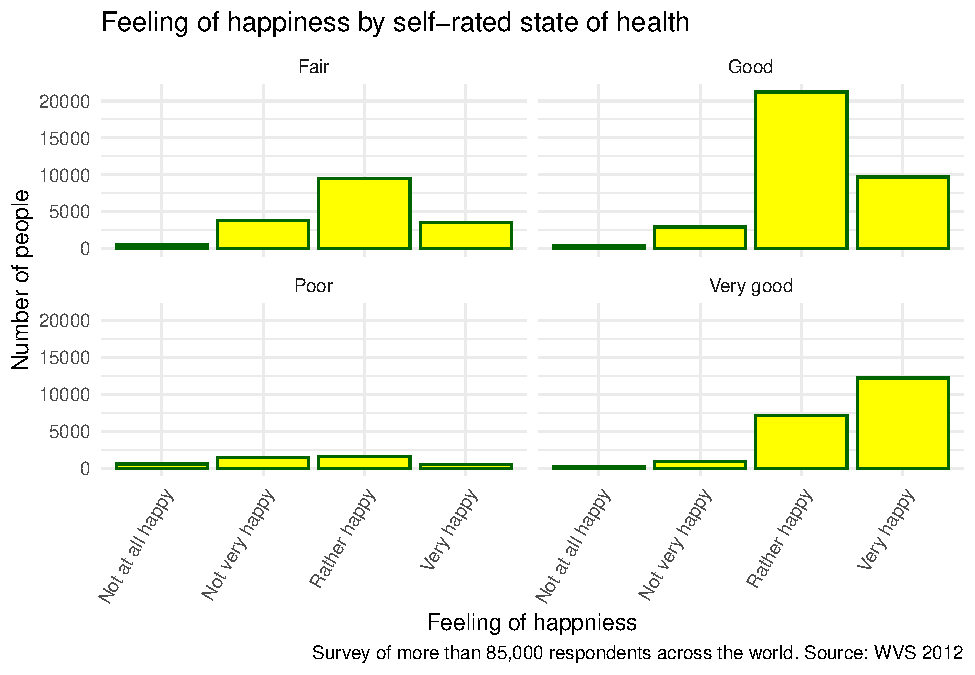
\includegraphics{610_final_files/figure-latex/trust and health-1.pdf}

\begin{tabular}{l|l|r}
\hline
most\_people\_trusted & feeling\_of\_happiness & n\\
\hline
Most people can be trusted & Not at all happy & 255\\
\hline
Most people can be trusted & Not very happy & 1528\\
\hline
Most people can be trusted & Rather happy & 10369\\
\hline
Most people can be trusted & Very happy & 6499\\
\hline
Need to be very careful & Not at all happy & 1368\\
\hline
Need to be very careful & Not very happy & 7619\\
\hline
Need to be very careful & Rather happy & 29072\\
\hline
Need to be very careful & Very happy & 19512\\
\hline
\end{tabular}

\begin{figure}
\centering
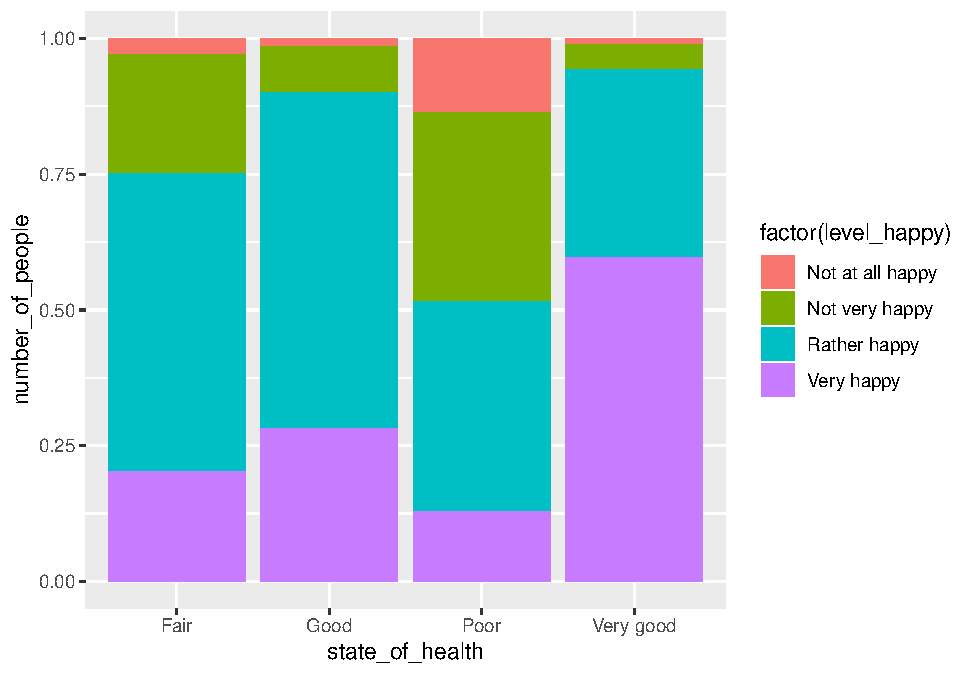
\includegraphics{610_final_files/figure-latex/trust and health-2.pdf}
\caption{}
\end{figure}

\subsection{Happiness and trust}\label{happiness-and-trust}

Out of the total 76222 people, only slightly more than 24.47 percent say
they can trust most of the people around them, while 75.53 is caucious
about the society.

See below
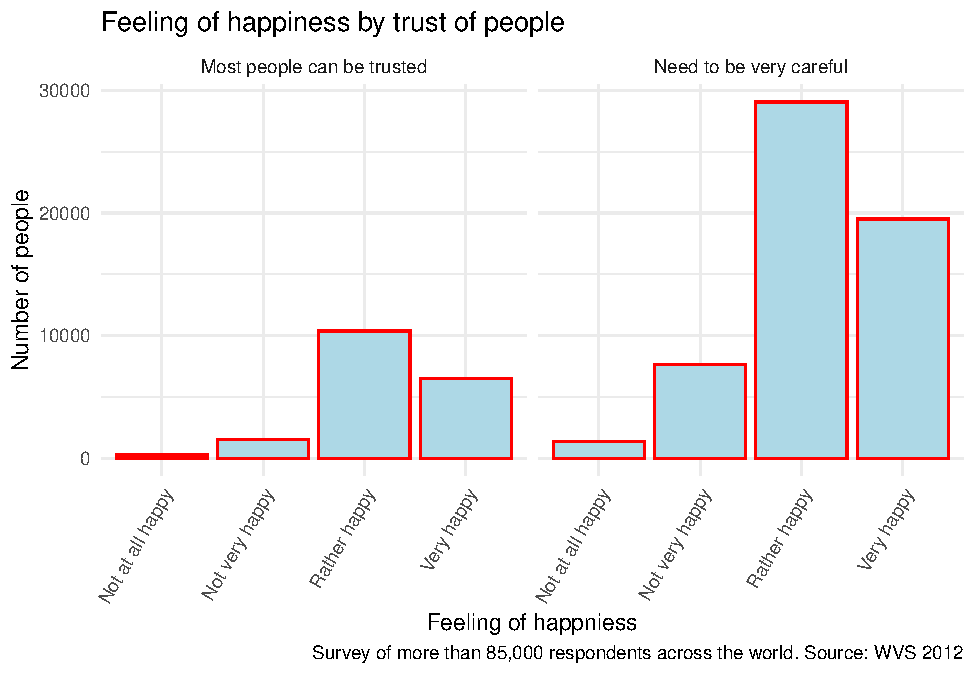
\includegraphics{610_final_files/figure-latex/unnamed-chunk-1-1.pdf} it
shows us

\section{Introduction}\label{introduction}

Study of happiness and its causal factors has been flourished in recent
years. This project explores the relationship between happiness and some
candidate variables, namely marital status, religious affiliation, level
of income, status of heath, and level of trust. We use individual level
survey of more than 85,000 respondents across 60 countries and societies
around the world in World Value Survey Dataset 2012.

Scholars have studied the relationship between happines and political
system (Inglehart, 2009)\ldots{}

Johnson (2012) finds that \enquote{trust as measured by the World Values
Survey is positively correlated with experimentally measured trust}.

Gandelman and Hernández-Murillo (2013) reviews relationship of self-rate
health status and perceived life quality.

\section{Methods}\label{methods}

We report how we determined our sample size, all data exclusions (if
any), all manipulations, and all measures in the study.

\subsection{Data analysis}\label{data-analysis}

We used R (Version 3.5.1; R Core Team, 2018) and the R-packages
\emph{dplyr} (Version 0.8.3; Wickham, François, Henry, \& Müller, 2019),
\emph{forcats} (Version 0.4.0; Wickham, 2019a), \emph{ggplot2} (Version
3.2.1; Wickham, 2016), \emph{here} (Version 0.1; Müller, 2017),
\emph{janitor} (Version 1.2.0; Firke, 2019), \emph{kableExtra} (Version
1.1.0; Zhu, 2019), \emph{knitr} (Version 1.25; Xie, 2015), \emph{papaja}
(Version 0.1.0.9842; Aust \& Barth, 2018), \emph{purrr} (Version 0.3.3;
Henry \& Wickham, 2019), \emph{readr} (Version 1.3.1; Wickham, Hester,
\& Francois, 2018), \emph{rio} (Version 0.5.16; C.-h. Chan, Chan,
Leeper, \& Becker, 2018), \emph{stringr} (Version 1.4.0; Wickham,
2019b), \emph{tibble} (Version 2.1.3; Müller \& Wickham, 2019),
\emph{tidyr} (Version 1.0.0; Wickham \& Henry, 2019), and
\emph{tidyverse} (Version 1.2.1; Wickham, 2017) for all our analyses.

\section{Results}\label{results}

\section{Discussion}\label{discussion}

\newpage

\section{References}\label{references}

\begingroup
\setlength{\parindent}{-0.5in} \setlength{\leftskip}{0.5in}

\hypertarget{refs}{}
\hypertarget{ref-R-papaja}{}
Aust, F., \& Barth, M. (2018). \emph{papaja: Create APA manuscripts with
R Markdown}. Retrieved from \url{https://github.com/crsh/papaja}

\hypertarget{ref-R-rio}{}
Chan, C.-h., Chan, G. C., Leeper, T. J., \& Becker, J. (2018).
\emph{Rio: A swiss-army knife for data file i/o}.

\hypertarget{ref-R-janitor}{}
Firke, S. (2019). \emph{Janitor: Simple tools for examining and cleaning
dirty data}. Retrieved from
\url{https://CRAN.R-project.org/package=janitor}

\hypertarget{ref-gandelman2013happiness}{}
Gandelman, N., \& Hernández-Murillo, R. (2013). What do happiness and
health satisfaction data tell us about relative risk aversion?
\emph{Journal of Economic Psychology}, \emph{39}, 301--312.

\hypertarget{ref-R-purrr}{}
Henry, L., \& Wickham, H. (2019). \emph{Purrr: Functional programming
tools}. Retrieved from \url{https://CRAN.R-project.org/package=purrr}

\hypertarget{ref-inglehart200911}{}
Inglehart, R. (2009). 11. democracy and happiness: What causes what?
\emph{Happiness, Economics and Politics: Towards a Multi-Disciplinary
Approach}, 256.

\hypertarget{ref-johnson2012much}{}
Johnson, N. D., \& Mislin, A. (2012). How much should we trust the world
values survey trust question? \emph{Economics Letters}, \emph{116}(2),
210--212.

\hypertarget{ref-R-here}{}
Müller, K. (2017). \emph{Here: A simpler way to find your files}.
Retrieved from \url{https://CRAN.R-project.org/package=here}

\hypertarget{ref-R-tibble}{}
Müller, K., \& Wickham, H. (2019). \emph{Tibble: Simple data frames}.
Retrieved from \url{https://CRAN.R-project.org/package=tibble}

\hypertarget{ref-R-base}{}
R Core Team. (2018). \emph{R: A language and environment for statistical
computing}. Vienna, Austria: R Foundation for Statistical Computing.
Retrieved from \url{https://www.R-project.org/}

\hypertarget{ref-R-ggplot2}{}
Wickham, H. (2016). \emph{Ggplot2: Elegant graphics for data analysis}.
Springer-Verlag New York. Retrieved from
\url{https://ggplot2.tidyverse.org}

\hypertarget{ref-R-tidyverse}{}
Wickham, H. (2017). \emph{Tidyverse: Easily install and load the
'tidyverse'}. Retrieved from
\url{https://CRAN.R-project.org/package=tidyverse}

\hypertarget{ref-R-forcats}{}
Wickham, H. (2019a). \emph{Forcats: Tools for working with categorical
variables (factors)}. Retrieved from
\url{https://CRAN.R-project.org/package=forcats}

\hypertarget{ref-R-stringr}{}
Wickham, H. (2019b). \emph{Stringr: Simple, consistent wrappers for
common string operations}. Retrieved from
\url{https://CRAN.R-project.org/package=stringr}

\hypertarget{ref-R-tidyr}{}
Wickham, H., \& Henry, L. (2019). \emph{Tidyr: Tidy messy data}.
Retrieved from \url{https://CRAN.R-project.org/package=tidyr}

\hypertarget{ref-R-dplyr}{}
Wickham, H., François, R., Henry, L., \& Müller, K. (2019). \emph{Dplyr:
A grammar of data manipulation}. Retrieved from
\url{https://CRAN.R-project.org/package=dplyr}

\hypertarget{ref-R-readr}{}
Wickham, H., Hester, J., \& Francois, R. (2018). \emph{Readr: Read
rectangular text data}. Retrieved from
\url{https://CRAN.R-project.org/package=readr}

\hypertarget{ref-R-knitr}{}
Xie, Y. (2015). \emph{Dynamic documents with R and knitr} (2nd ed.).
Boca Raton, Florida: Chapman; Hall/CRC. Retrieved from
\url{https://yihui.name/knitr/}

\hypertarget{ref-R-kableExtra}{}
Zhu, H. (2019). \emph{KableExtra: Construct complex table with 'kable'
and pipe syntax}. Retrieved from
\url{https://CRAN.R-project.org/package=kableExtra}

\endgroup

Final Paper

The final project must:

\begin{enumerate}
\def\labelenumi{(\alph{enumi})}
\tightlist
\item
  be a reproducible and dynamic APA manuscript produced with R Markdown,
  via the \{papaja\} package and include references to the extant
  literature;
\item
  be housed on GitHub, with contributions from all authors obvious;
\item
  demonstrate moving data from its raw \enquote{messy} format to a tidy
  data format through the R Markdown file, but not in the final
  document;
\item
  include at least two exploratory data visualizations, and
\item
  include at least summary statistics of the data in tables, although
  fitted models of any sort are an added bonus (not literally, there are
  not extra points for fitting a model).
\end{enumerate}

\subsection{The points for the final project are broken down as
follows:}\label{the-points-for-the-final-project-are-broken-down-as-follows}

\subsubsection{Writing (abstract, intro, methods, results, discussion,
references)}\label{writing-abstract-intro-methods-results-discussion-references}

\begin{itemize}
\tightlist
\item
  30 points(25\%) Document is fully reproducible and housed on GitHub
\item
  25 points (21\%) Demonstrate use of inline code
\item
  5 points (4\%) Demonstrate tidying messy data
\item
  30 points (25\%) Two data visualizations
\item
  20 points(10 points each) (17\%) Production of at least one table (of
  summary statistics or model results)
\item
  10 points (8\%)
\end{itemize}


\end{document}
